\documentclass{standalone}
\usepackage{tikz}
\usetikzlibrary{automata, positioning, arrows}

\begin{document}
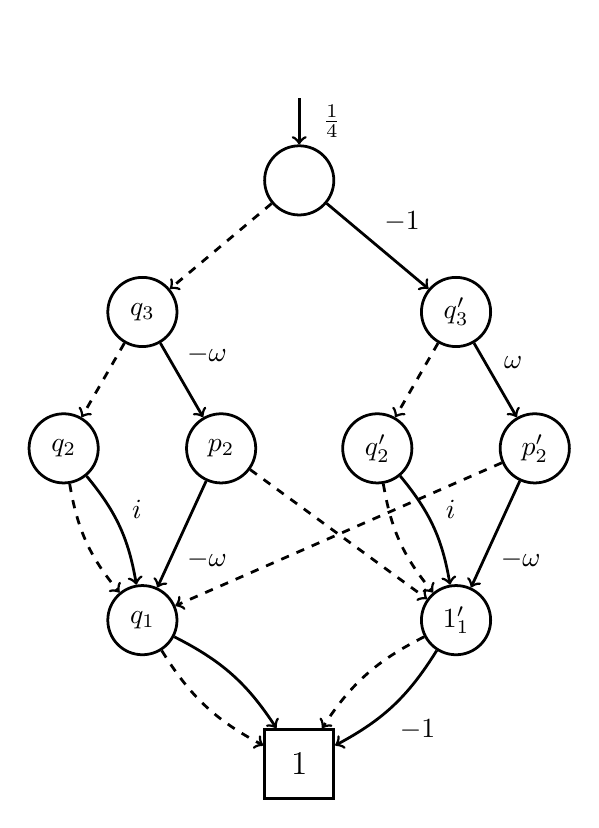
\begin{tikzpicture}[auto,node distance=1.5cm,every node/.style={shape=circle , align=center,solid,minimum size =0.01cm},line width =1pt]
  \tikzstyle{every state}=[fill=white,draw=black,text=black]

  \node[state] (A) {};
  \node[state] (B) at ([shift = ({220:2.6cm})]A) {$q_3$};
  \node[state] (C) at ([shift = ({-40:2.6cm})]A) {$q_3'$};
  \node[state] (D) at ([shift = ({240:2cm})]B) {$q_2$};
  \node[state] (E) at ([shift = ({-60:2cm})]B) {$p_2$};
  \node[state] (F) at ([shift = ({240:2cm})]C) {$q_2'$};
  \node[state] (G) at ([shift = ({-60:2cm})]C) {$p_2'$};
  \node[state] (D1) [below = 3cm of B] {$q_1$};
  \node[state] (F1) [below = 3cm of C] {$1_1'$};
  \node[state,shape = rectangle] (T) [below = 6.5cm of A] {\large$1$};
  \node[state,draw=none] (I) [above of= A]       {};

  \path[->]
  (A) edge[dashed]  node {} (B)
  (A) edge  node {$-1$} (C)
  (B) edge[dashed]  node {} (D)
  (B) edge  node {$-\omega$} (E)
  (C) edge[dashed]  node {} (F)
  (C) edge  node {$\omega$} (G)
  (D) edge[dashed, bend right = 15] node {} (D1)
  (D) edge[bend left = 15] node {$i$} (D1)
  (E) edge node {$-\omega$} (D1)
  (E) edge[dashed] node {} (F1)
  (F) edge[dashed, bend right=15] node {} (F1)
  (F) edge[bend left=15] node {$i$} (F1)
  (G) edge[dashed] node {} (D1)
  (G) edge node {$-\omega$} (F1)
  (D1) edge[dashed, bend right = 15] node {} (T)
  (D1) edge[bend left = 15] node {} (T)
  (F1) edge[dashed, bend right = 15] node {} (T)
  (F1) edge[bend left = 15] node {$-1$} (T)
  (I) edge node{$\frac{1}{4}$} (A);

\end{tikzpicture}
\end{document}